\section{Generative Agent Architecture}\label{sec:architecture}
Generative agents aim to provide a framework for behavior in an open world: one that can engage in interactions with other agents and react to changes in the environment. Generative agents take their current environment and past experiences as input and generate behavior as output. Underlying this behavior is a novel agent architecture that combines a large language model with mechanisms for synthesizing and retrieving relevant information to condition the language model's output. Without these mechanisms, large language models can output behavior, but the resulting agents may not react based on the agent's past experiences, may not make important inferences, and may not maintain long-term coherence. Challenges with long-term planning and coherence remain~\cite{bubeck2023sparks} even with today's most performant models such as GPT-4. Because generative agents produce large streams of events and memories that must be retained, a core challenge of our architecture is to ensure that the most relevant pieces of the agent's memory are retrieved and synthesized when needed.

At the center of our architecture is the memory stream, a database that maintains a comprehensive record of an agent's experience. From the memory stream, records are retrieved as relevant to plan the agent's actions and react appropriately to the environment. Records are recursively synthesized into higher- and higher-level reflections that guide behavior. Everything in the architecture is recorded and reasoned over as a natural language description, allowing the architecture to leverage a large language model.

Our current implementation utilizes the gpt3.5-turbo version of ChatGPT~\cite{openai_chatgpt}. We expect that the architectural basics of generative agents---memory, planning, and reflection---will likely remain the same as language models improve. Newer language models (e.g., GPT-4) will continue to expand the expressive power and performance of the prompts that underpin generative agents. As of writing, however, GPT-4's API was invitation-only, so our agents use ChatGPT.

\begin{figure*}[tb]
  \centering
  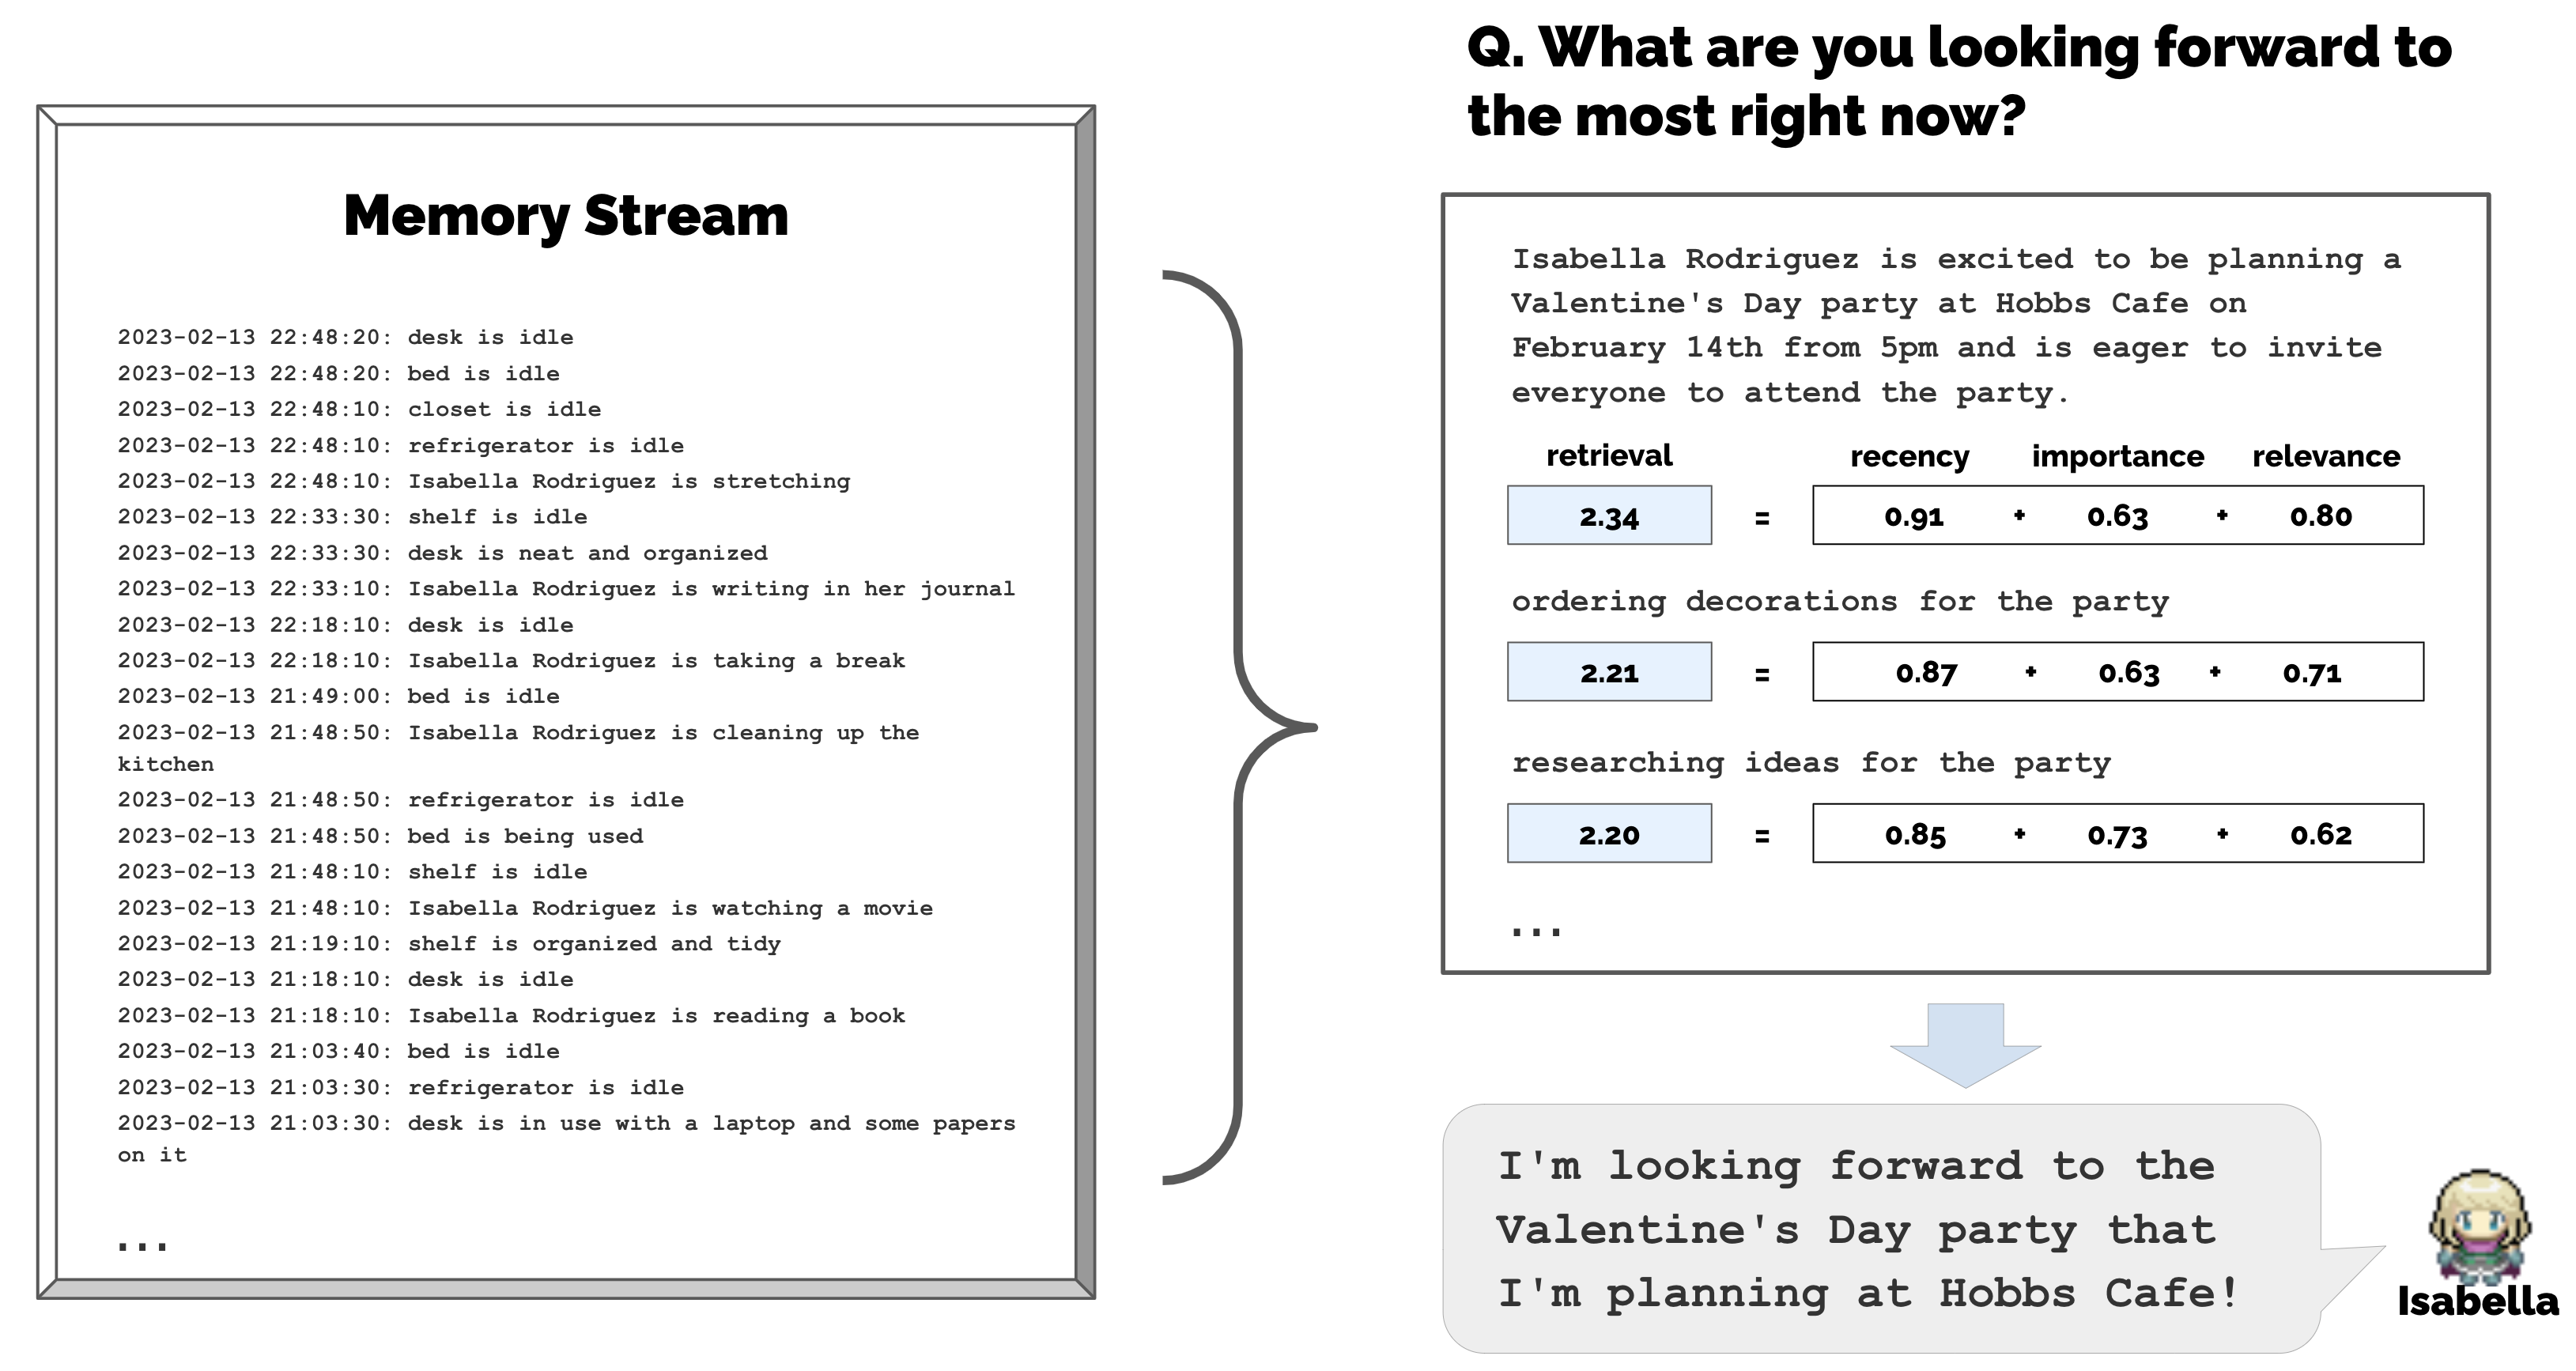
\includegraphics[width=0.86\textwidth]{figures/figure_retrieval2.png}
  \caption{The memory stream comprises a large number of observations that are relevant and irrelevant to the agent's current situation. Retrieval identifies a subset of these observations that should be passed to the language model to condition its response to the situation.}
  \Description{On the left, a large list of events such as ``refrigerator is idle''. On the right, the question ``What are you looking forward to the most right now?'', followed by retrieval calculations that rank ``ordering decorations for the party'' and ``researching ideas for the party'' highly. Based on these memories, Isabella responds, ``I'm looking forward to the Valentine's Day party that I'm planning at Hobbs Cafe!''}
  \label{fig:retrieval_function}
\end{figure*}

\subsection{Memory and Retrieval}

\subsubsection*{Challenge:} Creating generative agents that can simulate human behavior requires reasoning about a set of experiences that is far larger than what should be described in a prompt, as the full memory stream can distract the model and does not even currently fit into the limited context window. Consider the Isabella agent answering the question, ``What are you passionate about these days?'' Summarizing all of Isabella's experiences to fit in the limited context window of the language model produces an uninformative response, where Isabella discusses topics such as collaborations for events and projects and cleanliness and organization in a cafe. Instead of summarizing, the memory stream described below surfaces relevant memories, resulting in a more informative and specific response that mentions Isabella's passion for making people feel welcome and included, planning events and creating an atmosphere that people can enjoy, such as the Valentine's Day party.

\subsubsection*{Approach:}
The \textit{memory stream} maintains a comprehensive record of the agent's experience. It is a list of memory objects, where each object contains a natural language description, a creation timestamp, and a most recent access timestamp. The most basic element of the memory stream is an \textit{observation}, which is an event directly perceived by an agent. Common observations include behaviors performed by the agent themselves or behaviors that agents perceive being performed by other agents or non-agent objects. For instance, Isabella Rodriguez, who works at a coffee shop, might accrue the following observations over time: (1)~\gentxt{Isabella Rodriguez is setting out the pastries}, (2)~\gentxt{Maria Lopez is studying for a Chemistry test while drinking coffee}, (3)~\gentxt{Isabella Rodriguez and Maria Lopez are conversing about planning a Valentine's day party at Hobbs Cafe}, (4)~\gentxt{The refrigerator is empty}.

Our architecture implements a retrieval function that takes the agent's current situation as input and returns a subset of the memory stream to pass on to the language model. There are many possible implementations of a retrieval function, depending on what is important for the agent to consider when deciding how to act. In our context, we focus on three main components that, together, produce effective results.

\textit{Recency} assigns a higher score to memory objects that were recently accessed, so that events from a moment ago or this morning are likely to remain in the agent's attentional sphere. In our implementation, we treat recency as an exponential decay function over the number of sandbox game hours since the memory was last retrieved. Our decay factor is $0.995$. 

\textit{Importance} distinguishes mundane from core memories by assigning a higher score to memory objects that the agent believes to be important. For instance, a mundane event, such as eating breakfast in one's room, would yield a low importance score, whereas a breakup with one's significant other would yield a high score. There are many possible implementations of an importance score; we find that directly asking the language model to output an integer score is effective. The full prompt appears below:
    \begin{quote}
    {\small
    \texttt{On the scale of 1 to 10, where 1 is purely mundane (e.g., brushing teeth, making bed) and 10 is extremely poignant (e.g., a break up, college acceptance), rate the likely poignancy of the following piece of memory.\\
    Memory: buying groceries at The Willows Market and Pharmacy\\
    Rating: <fill in>}
    }
    \end{quote}
This prompt returns an integer value of \gentxt{2} for “cleaning up the room” and \gentxt{8} for “asking your crush out on a date.” The importance score is generated at the time the memory object is created.

\textit{Relevance} assigns a higher score to memory objects that are related to the current situation. What is relevant depends on the answer to, ``Relevant to what?'', so we condition relevance on a \textit{query} memory. If the query, for example, is that a student is discussing what to study for a chemistry test with a classmate, memory objects about their breakfast should have low relevance, whereas memory objects about the teacher and schoolwork should have high relevance. In our implementation, we use the language model to generate an embedding vector of the text description of each memory. Then, we calculate relevance as the cosine similarity between the memory's embedding vector and the query memory's embedding vector.

To calculate the final retrieval score, we normalize the recency, relevance, and importance scores to the range of $[0, 1]$ using min-max scaling. The retrieval function scores all memories as a weighted combination of the three elements: $score=\alpha_{recency} \cdot recency + \alpha_{importance} \cdot importance + \alpha_{relevance} \cdot relevance$. In our implementation, all $\alpha$s are set to 1. The top-ranked memories that fit within the language model's context window are included in the prompt.


\subsection{Reflection}

\begin{figure*}[tb]
  \centering
  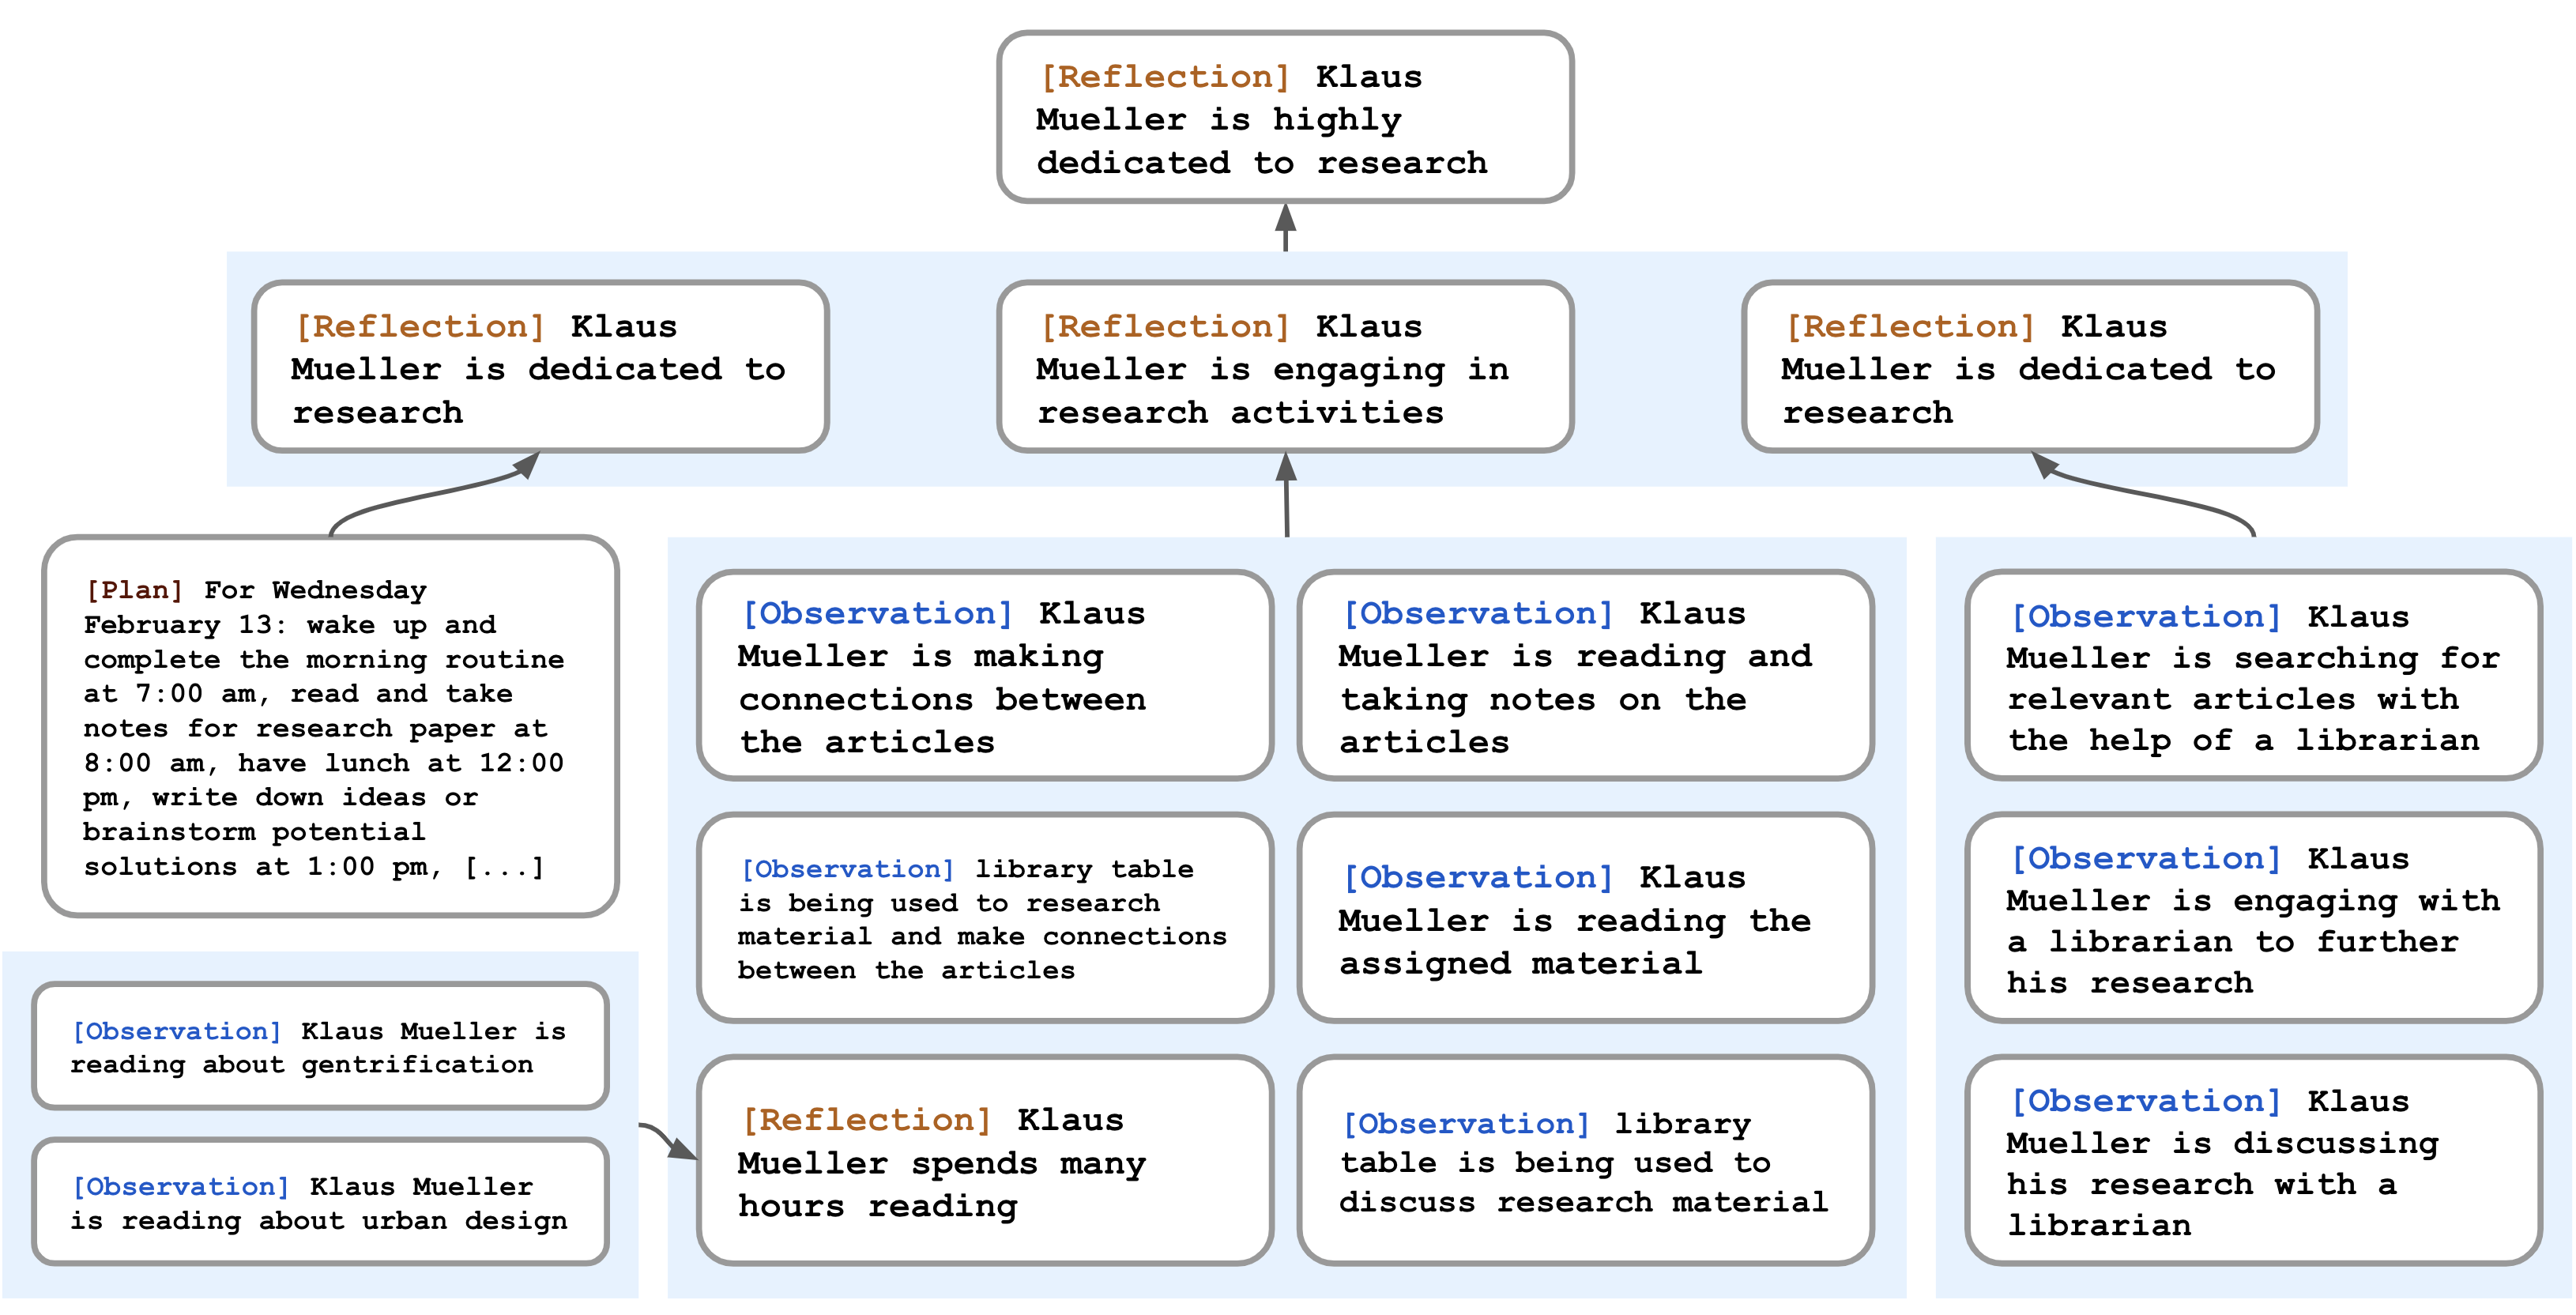
\includegraphics[width=0.92\textwidth]{figures/figure_reflection6.png}
  \caption{A reflection tree for Klaus Mueller. The agent's observations of the world, represented in the leaf nodes, are recursively synthesized to derive Klaus's self-notion that he is highly dedicated to his research. }
  \Description{The reflection tree.}
  \label{fig:reflection_tree}
\end{figure*}





\subsubsection*{Challenge:} Generative agents, when equipped with only raw observational memory, struggle to generalize or make inferences. Consider a scenario in which Klaus Mueller is asked by the user: ``If you had to choose one person of those you know to spend an hour with, who would it be?" With access to only observational memory, the agent simply chooses the person with whom Klaus has had the most frequent interactions: Wolfgang, his college dorm neighbor. Unfortunately, Wolfgang and Klaus only ever see each other in passing, and do not have deep interactions. A more desirable response requires that the agent generalize from memories of Klaus spending hours on a research project to generate a higher-level reflection that Klaus is passionate about research, and likewise recognize Maria putting in effort into her own research (albeit in a different field), enabling a reflection that they share a common interest. With the approach below, when Klaus is asked who to spend time with, Klaus chooses Maria instead of Wolfgang. 

\subsubsection*{Approach: } We introduce a second type of memory, which we call a \textit{reflection}. Reflections are higher-level, more abstract thoughts generated by the agent. Because they are a type of memory, they are included alongside other observations when retrieval occurs. Reflections are generated periodically; in our implementation, we generate reflections when the sum of the importance scores for the latest events perceived by the agents exceeds a threshold (150 in our implementation). In practice, our agents reflected roughly two or three times a day.

The first step in reflection is for the agent to determine what to reflect on, by identifying questions that can be asked given the agent's recent experiences. We query the large language model with the 100 most recent records in the agent's memory stream (e.g., ``Klaus Mueller is reading a book on gentrification'', ``Klaus Mueller is conversing with a librarian about his research project'', ``desk at the library is currently unoccupied'') and prompt the language model, ``Given only the information above, what are 3 most salient high-level questions we can answer about the subjects in the statements?'' The model's response generates candidate questions: for example, \gentxt{What topic is Klaus Mueller passionate about?} and \gentxt{What is the relationship between Klaus Mueller and Maria Lopez?} We use these generated questions as queries for retrieval, and gather relevant memories (including other reflections) for each question. Then we prompt the language model to extract insights and cite the particular records that served as evidence for the insights. The full prompt is as follows:
\begin{quote}
    {\small
    \texttt{Statements about Klaus Mueller \\
            1. Klaus Mueller is writing a research paper  \\
            2. Klaus Mueller enjoys reading a book \\on gentrification \\
            3. Klaus Mueller is conversing with Ayesha Khan about exercising [...]\\
            What 5 high-level insights can you infer from the above statements? (example format: insight (because of 1, 5, 3))
            }
    }
\end{quote}
This process generates statements such as \gentxt{Klaus Mueller is dedicated to his research on gentrification (because of 1, 2, 8, 15)}. We parse and store the statement as a reflection in the memory stream, including pointers to the memory objects that were cited. 

Reflection explicitly allows the agents to reflect not only on their observations but also on other reflections: for example, the second statement about Klaus Mueller above is a reflection that Klaus previously had, not an observation from his environment. As a result, agents generate trees of reflections: the leaf nodes of the tree represent the base observations, and the non-leaf nodes represent thoughts that become more abstract and higher-level the higher up the tree they are.

\subsection{Planning and Reacting}

\subsubsection*{Challenge:}
While a large language model can generate plausible behavior in response to situational information~(e.g.,~\cite{9_park2022socialsimulacra,63_horton2023large}), agents need to plan over a longer time horizon to ensure that their sequence of actions is coherent and believable. If we prompt a language model with Klaus's background, describe the time, and ask what action he ought to take at the given moment, Klaus would eat lunch at 12 pm, but then again at 12:30 pm and 1 pm, despite having already eaten his lunch twice. Optimizing for believability in the moment sacrifices believability over time. To overcome this issue, planning is essential. With the approach described below, Klaus's afternoon plan is less gluttonous: he has lunch at Hobbs Cafe while reading at 12pm, works on his research paper at the school library at 1pm, and takes a break for a walk in the park at 3pm.

\subsubsection*{Approach:}
Plans describe a future sequence of actions for the agent, and help keep the agent's behavior consistent over time. A plan includes a location, a starting time, and a duration. For instance, Klaus Mueller, who is \gentxt{dedicated in his research} and has an impending deadline,\footnote{And, in this way, bears at least a passing resemblance to the authors of this paper.} may choose to spend his day working at his desk drafting his research paper. An entry in a plan might state, for example: \gentxt{for 180 minutes from 9am, February 12th, 2023, at Oak Hill College Dorm: Klaus Mueller’s room: desk, read and take notes for research paper}. Like reflections, plans are stored in the memory stream and are included in the retrieval process. This allows the agent to consider observations, reflections, and plans all together when deciding how to behave. Agents may change their plans midstream if needed.

It would be unrealistic and uninteresting for an artist agent to plan on painting while sitting at a pharmacy counter for four hours without moving. A more desirable plan would involve the agent taking the necessary time to gather materials, mix paint, take breaks, and clean up during the four-hour period in their home studio. To create such plans, our approach starts top-down and then recursively generates more detail. The first step is to create a plan that outlines the day's agenda in broad strokes. To create the initial plan, we prompt the language model with the agent's summary description (e.g., name, traits, and a summary of their recent experiences) and a summary of their previous day. A full example prompt is below, which is unfinished at the bottom for the language model to complete:
\begin{quote}
    {\small
    \texttt{Name: Eddy Lin (age: 19) \\
        Innate traits: friendly, outgoing, hospitable\\
        Eddy Lin is a student at Oak Hill College studying music theory and composition. He loves to explore different musical styles and is always looking for ways to expand his knowledge. Eddy Lin is working on a composition project for his college class. He is taking classes to learn more about music theory. Eddy Lin is excited about the new composition he is working on but he wants to dedicate more hours in the day to work on it in the coming days\\
        On Tuesday February 12, Eddy 1) woke up and completed the morning routine at 7:00 am, […] 6) got ready to sleep around 10 pm.\\
        Today is Wednesday February 13. Here is Eddy’s plan today in broad strokes: 1)
    }
    }
\end{quote}
This generates a rough sketch of the agent's plan for a day, divided into five to eight chunks: “\gentxt{1) wake up and complete the morning routine at 8:00 am, 2) go to Oak Hill College to take classes starting 10:00 am, […] 5) work on his new music composition from 1:00 pm to 5:00 pm, 6) have dinner at 5:30 pm, 7) finish school assignments and go to bed by 11:00 pm.}” 

The agent saves this plan in the memory stream and then recursively decomposes it to create finer-grained actions, first into hour-long chunks of actions---Eddy’s plan to \gentxt{work on his new music composition from 1:00 pm to 5:00 pm} becomes \gentxt{1:00 pm: start by brainstorming some ideas for his music composition [...] 4:00 pm: take a quick break and recharge his creative energy before reviewing and polishing his composition}. We then recursively decompose this again into 5--15 minute chunks: e.g., \gentxt{4:00 pm: grab a light snack, such as a piece of fruit, a granola bar, or some nuts. 4:05 pm: take a short walk around his workspace [...] 4:50 pm: take a few minutes to clean up his workspace}. This process can be adjusted to match the desired granularity. 

\subsubsection{Reacting and Updating Plans}
Generative agents operate in an action loop where, at each time step, they perceive the world around them and those perceived observations are stored in their memory stream. We prompt the language model with these observations to decide whether the agent should continue with their existing plan, or react. Standing at an easel and painting, for example, might trigger an observation of the easel, but this is unlikely to prompt a reaction. However, if Eddy's father John records that he sees Eddy taking a short walk in the house garden, the outcome is different. The prompt is below, with \texttt{[Agent's Summary Description]} standing in for a dynamically-generated, paragraph-long summary of the agent's overall goals and disposition, which is described in Appendix~\ref{sec:optimization}:
\begin{quote}
    {\small
    \texttt{[Agent's Summary Description]\\
            It is February 13, 2023, 4:56 pm. \\
            John Lin’s status: John is back home early from work. \\
            Observation: John saw Eddy taking a short walk around his workplace.\\
            Summary of relevant context from John’s memory: Eddy Lin is John’s Lin’s son. Eddy Lin has been working on a music composition for his class. Eddy Lin likes to walk around the garden when he is thinking about or listening to music.\\
            Should John react to the observation, and if so, what would be an appropriate reaction?
    }
    }
\end{quote}
The context summary is generated through two prompts that retrieve memories via the queries ``What is [observer]’s relationship with the [observed entity]?'' and ``[Observed entity] is [action status of the observed entity]'', and their answers summarized together. The output suggests that \gentxt{John could consider asking Eddy about his music composition project}. We then regenerate the agent's existing plan starting from the time when the reaction takes place. Finally, if the action indicates an interaction between agents, we generate their dialogue.

\subsubsection{Dialogue}
Agents converse as they interact with each other. We generate agents' dialogue by conditioning their utterances on their memories about each other. For example, when John initiates his conversation with Eddy, we generate John's first utterance by using his summarized memory about Eddy and the intended reaction when he decided to ask Eddy about his composition project:
\begin{quote}
    {\small
    \texttt{[Agent’s Summary Description]\\
            It is February 13, 2023, 4:56 pm.\\ 
            John Lin’s status: John is back home early from work.\\ 
            Observation: John saw Eddy taking a short walk around his workplace.\\
            Summary of relevant context from John’s memory: Eddy Lin is John’s Lin’s son. Eddy Lin has been working on a music composition for his class. Eddy Lin likes to walk around the garden when he is thinking about or listening to music.\\
            John is asking Eddy about his music composition \\project. What would he say to Eddy?}
    }
\end{quote}
The result: \gentxt{``Hey Eddy, how's the music composition project for your class coming along?''} From Eddy's perspective, John initiating the dialogue is seen as an event to which he may want to react. So, just as John did, Eddy retrieves and summarizes his memory about his relationship with John, as well as his memory that may be related to John's last utterance in the dialogue. If he decides to respond, we generate Eddy's utterance using his summarized memory and the current dialogue history:
\begin{quote}
    {\small
    \texttt{[Agent’s Summary Description]\\
            It is February 13, 2023, 4:56 pm.\\
            Eddy Lin’s status: Eddy is taking a short walk around his workplace.\\
            Observation: John is initiating a conversation with Eddy.\\
            Summary of relevant context from Eddy’s memory: John Lin is Eddy Lin’s father. John Lin is caring and is interested to learn more about Eddy Lin’s school work. John Lin knows that Eddy Lin is working on a music composition. \\
            Here is the dialogue history: \\
            John: Hey Eddy, how's the music composition project for your class coming along? \\
            How would Eddy respond to John?}
    }
\end{quote}
This generates Eddy's response: \gentxt{``Hey Dad, it's going well. I've been taking walks around the garden to clear my head and get some inspiration.''} The continuation of this dialogue is generated using the same mechanism until one of the two agents decides to end the dialogue.

